\NeedsTeXFormat{LaTeX2e}
\documentclass[12pt,a4paper]{article}
\usepackage{german,a4}
\usepackage{epsfig}
\begin{document}

%%% TITLE =============================================================

\begin{titlepage}

\vspace*{\fill}
\begin{center}
\Huge{\bf{Ein Browser f\"ur Alice}}   
\end{center}

\vspace{1cm}

\center{\large{\today}}

\vspace{1cm}

\begin{center}
  \begin{minipage}[center]{10cm}
    \begin{tabbing} 
      \large{Bernadette Blum} \hspace{1cm}\= \large{Marvin Schiller}\\
      blum@ps.uni-sb.de \> schiller@ps.uni-sb.de\\[1cm]

      Betreuer: \\[2mm]
      Thorsten Brunklaus \> Andreas Rossberg\\
      \small{brunklaus@ps.uni-sb.de} \> \small{rossberg@ps.uni-sb.de}\\[5mm]


      Leitung: \\
      Prof. Dr. Gert Smolka \> \small Fachbereich Informatik \\ 
      \small{smolka@ps.uni-sb.de} \> \small Universit\"{a}t des Saarlandes\\ 
    \> \small Im Stadtwald \\
    \> \small  66123 Saarbr\"{u}cken \\[5mm]

    \end{tabbing}
  \end{minipage}
\end{center}



\vspace*{\fill}

\normalsize
\end{titlepage}


\begin{abstract}

Dieser Bericht zeigt Design und Implementierung eines 
interaktiven Browser-Tools f\"{u}r die funktionale Programmiersprache 
Alice. Da Alice-Werte nicht selbstbeschreibend sind, 
muss der Browser jeweils explizite Typinformationen zu denjenigen  
Werten erhalten, die dargestellt werden sollen. 
Um Werte abstrakter Typen in eine entsprechende Darstellung 
transformieren zu k\"{o}nnen, wird weiterhin 
deren Registrierung beim Browser erforderlich. 
Der Browser ist in Alice selbst implementiert und verwendet die Gtk-Bibliothek
zur Erzeugung der graphischen Benutzerschnittstelle.
Unser Design kn\"{u}pft weitgehend an Thorsten Brunklaus' ''Oz Inspektor'' 
\cite{br:oz} an.

\end{abstract}


%%% EINFUEHRUNG ==========================================================

\section{Einf\"{u}hrung}  

\paragraph{}

Die graphische Aufbereitung von Programmen und Datenstrukturen erm\"{o}glicht 
Programmierern das Debuggen komplexer Programme. 
Dazu werden Algorithmen entwickelt, die man als ``Pretty Printer'' bezeichnet. 
Ziel bei der Entwicklung von Pretty Printern ist es, die Lesbarkeit eines 
Dokuments (meist Programme und mathematische Ausdr\"{u}cke) durch 
Einr\"{u}ckungen, gezielte Zeilenumbr\"{u}che und 
visuelle Attribute zu verbessern.
Dieser Bericht stellt Design und Implementierung 
eines solchen ``Pretty Printers'' f\"{u}r die Programmiersprache Alice vor. 

\paragraph{}

Die funktionale Programmiersprache Alice erm\"{o}glicht nebenl\"{a}ufige 
Programmierung und die Erzeugung zyklischer Datenstrukturen. 
Dies erlaubt es dem Programmierer, Berechnungsstr\"{a}nge (sog. Threads) 
willk\"{u}rlich zu starten oder zu beenden, Werte erst bei 
Bedarf auswerten zu lassen (sog. Laziness), oder Platzhalter 
f\"{u}r noch nicht bekannte Berechnungsergebnisse einzusetzen (sog. Futures).
\\
Die daraus resultierende Komplexit\"{a}t erfordert eine Darstellung, 
die diesen Konzepten in \"{U}bersichtlichkeit und Flexibilit\"{a}t gerecht 
wird.

\paragraph{}

Anders als beispielsweise in der Programmiersprache Oz sind 
Typen in Alice nicht selbstbeschreibend. Dadurch muss zur 
graphischen Darstellung eines Alice-Wertes durch den 
Browser nicht nur 
der Wert selbst, sondern auch strukturelle 
Information zu diesem Wert \"{u}bergeben werden. Diese l\"{a}sst sich durch 
sogenannte Typreflektion gewinnen. Dieser Bericht zeigt, 
wie im Browser die strukturelle Information 
bei der Darstellung der dazugeh\"{o}rigen Werte verwendet wird und 
welche Mechanismen n\"{o}tig sind, um Werte beliebiger abstrakter Typen 
darstellen zu k\"{o}nnen.


%%% ZENTRALE IDEEN =====================================================

\section{Zentrale Ideen}

\begin{center}
\begin{picture}(360,470)
\put(0,370){\framebox(360,100){\begin{math}
                                \begin{array}{clcr}
                                  (
                                  \{
                                   eins $=$ \sharp ''1'' ,
                                  zwei $=$ \sharp ''2'' \} , 
                                  \{ drei $=$  3 , 
                                  vier $=$  4 \} ) \\ 
                                  \bf{+}   \\
                                   Typreflektion 
                                  ( \{eins: char, zwei: char\},
                                  \{drei: int, vier: int\} )
                                \end{array}  
                                \end{math}}}
\put(180,360){\vector(0,-4){30}}
\put(80,220){\framebox(200,100){Browser-interne Wertbeschreibung}}
\put(180,210){\vector(0,-4){30}}
\put(40,0){
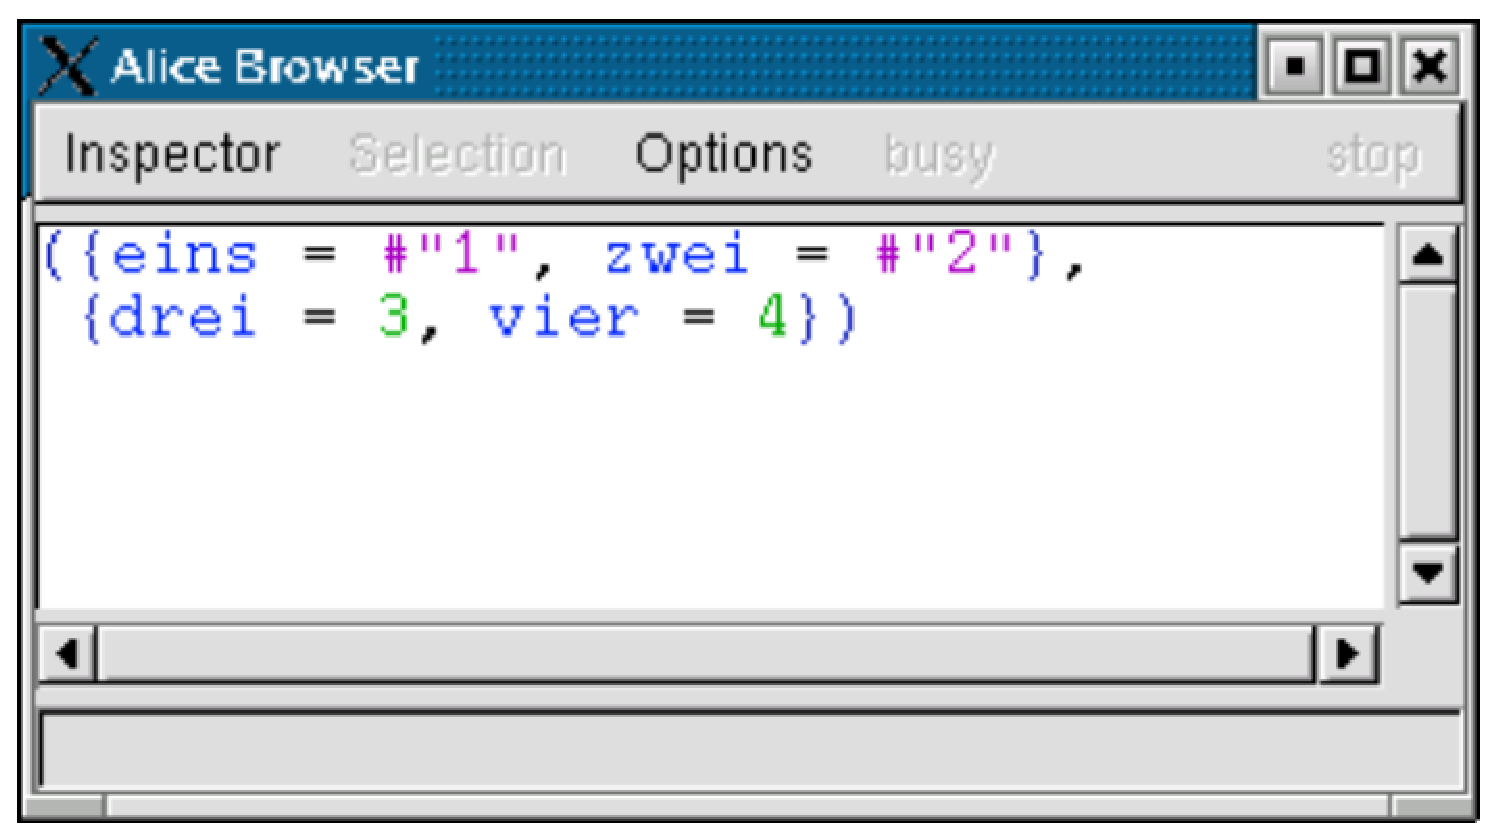
\epsfig{file = 3stepsgui.ps, width=10cm}}
\end{picture}
\newline
\nopagebreak
Abbildung 2.1: Vom Wert zur Browserdarstellung
\end{center}

Der Browser soll in der Lage sein, Alice-Werte 
\"ubersichtlich auf einer graphischen Benutzeroberfl\"ache  darzustellen. 
Dies wird erreicht, indem die Werte in eine interne Beschreibung 
transformiert werden, aus der die graphische Repr\"asentation 
erzeugt werden kann. Abbildung 2.1 verdeutlicht diesen Vorgang. 
Die Transformation in die interne Beschreibung wird durch die 
Typinformation der zu inspizierenden Werte gesteuert. 


\subsection{Typregistrierung}

\paragraph{}

Die Typen von Alice-Werten k\"onnen strukturelle oder abstrakte Typen 
sein. Um die Werte in eine entsprechende Darstellung transformieren 
zu k\"onnen, ben\"otigt der Browser explizite strukturelle  
Information zu diesen Werten. 

\paragraph{}

Gleichzeitig ben\"otigt der Browser Anweisungen, wie 
ein Wert eines bestimmten Typs in die interne 
Repr\"asentation und letztendlich die graphische Darstellung 
umgewandelt werden soll.

\paragraph{}

W\"ahrend strukturelle Typen die ben\"otigte Strukturinformation 
zu dieser Transformation liefern, m\"ussen abstrakte Typen 
zusammen mit passenden Darstellungsanweisungen beim Browser 
registriert werden. 
Diese Darstellungsvorschriften werden in Form einer 
Prozedur \"ubermittelt, welche die Umwandlung des Wertes in eine 
Wertbeschreibung spezifiziert.  

\subsection{Darstellungskriterien}

\paragraph{}

Der Entwurf eines graphischen Tools erfordert die \"Uberlegung, 
welche Kriterien bei der Wahl von Anordnungsvorschriften f\"ur 
die Darstellung der Datenstrukturen im Vordergrund stehen sollen. 
Es gibt Pretty Printer, die, wie auch der 
Algorithmus von Oppen \cite{op:pr}, die Einhaltung einer vorgegebenen 
darstellbaren Seitenbreite sicherstellen, und durch gezielte 
Umbr\"uche und Einr\"uckungen die Lesbarkeit wiederherstellen. Im 
Gegensatz dazu steht die Vorgehensweise, die Anordnung nicht 
an einer vorgegebenen Seitenbreite zu orientieren, sondern 
vielmehr die Gr\"o\ss e des Darstellungsbrereichs an eine m\"oglichst 
\"ubersichtliche Darstellung anzupassen. 
Im Fall des Alice-Browsers wurde letztere Vorgehensweise gew\"ahlt, 
um trotz der Komplexit\"at der Alice-Datenstrukturen 
eine klare Darstellung zu erm\"oglichen.

\paragraph{}

Zusammengesetzte Alice-Werte lassen sich in Teilwerte untergliedern, 
so dass sich ein solcher Wert 
in eine baumartige Darstellung zerlegen l\"asst.
Hier deutet sich schon an, 
dass sich auch die interne Behandlung der Datenstrukturen 
an Baumstrukturen orientieren muss. Gleichzeitig soll der Browser 
bei der graphischen Darstellung auf 
die f\"ur Alice \"ubliche Notation f\"ur 
Werte mit Klammern und Trennzeichen 
zur\"uck greifen.    
Die Darstellung von baumartigen Werten durch 
den Browser orientiert sich dabei 
an einer Regel, wie sie u.a. Kennedy \cite{ke:dr} f\"ur 
das Baumzeichnen aufstellt: Gleiche Teilb\"aume werden 
gleich dargestellt. 


%%% ENTWURF ============================================================

\section{Entwurf}

\begin{center}
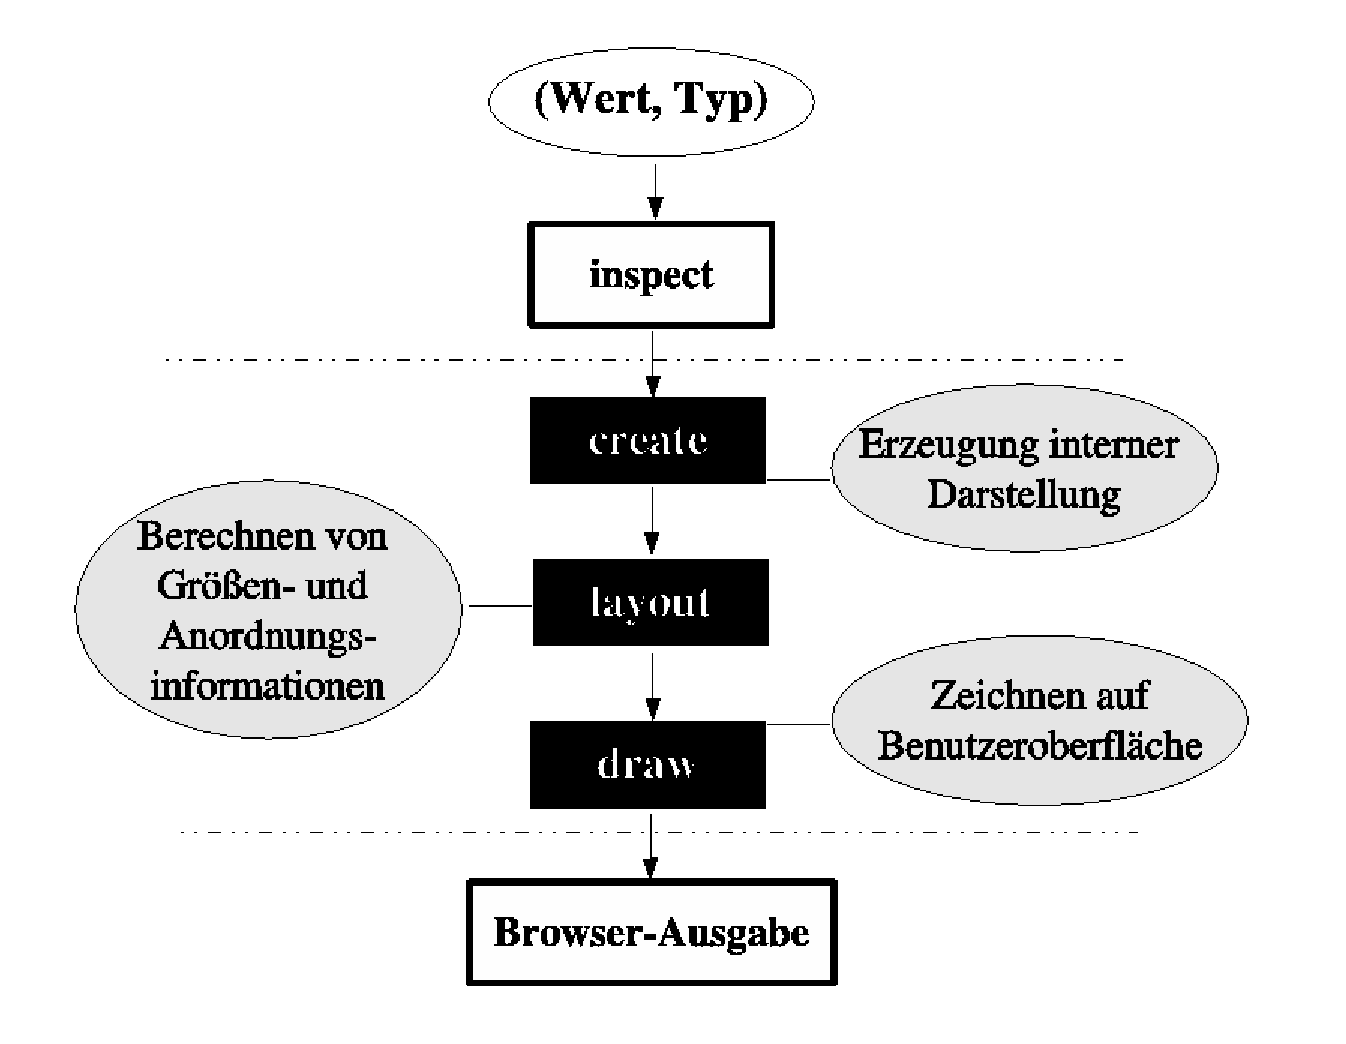
\epsfig{file = cld.ps, width = 13cm}
Abbildung 3.1: dreistufige Darstellungserzeugung
\end{center}

\paragraph{}

Abbildung 3.1 zeigt die dreistufige Erzeugung der graphischen
Wertdarstellung.Vom Benutzer wird die inspect-Funktion des 
Browsers aufgerufen.
Da Alice-Werte nicht selbstbeschreibend sind, ben\"otigt die
inspect-Funktion explizite Typinformation des zu inspizierenden
Wertes. Mithilfe eines Typreflektors wird diese Information
generiert und zusammen mit dem Wert an die inspect-Funktion
\"ubergeben. Um von dem Wert-Typ-Paar zur graphischen 
Darstellung des Wertes auf der Benutzeroberfl\"ache zu gelangen,
m\"ussen drei Phasen durchlaufen werden.

\paragraph{}

Zuerst eird eine interne Beschreibung des Wertes erzeugt, die
wichtige Informationen \"uber dessen Struktur enth\"alt. Diese
Phase wird Create-Phase genannt.

\paragraph{}    

In der nun folgenden Layout-Phase werden die Ma\ss e der 
Textrepr\"asentation des darzustellenden Wertes sowie 
all seiner Teilwerte berechnet. Dies dient zur Anordnung 
der Textrepr\"asentationen auf der Benutzeroberfl\"ache.

\paragraph{}

Im letzten Schritt wird die graphische Repr\"asentation 
unter Nutzung der durch das Layout berechneten Anordnungsinformation 
auf die graphische Benutzeroberfl\"ache gezeichnet. 

\subsection{Interne Darstellung}

\label{intern}

F\"ur die interne Darstellung von Werten als B\"aume ben\"otigen wir einen 
Typen. Dieser wird in Abbildung 3.2 dargestellt.\\[1mm]

\begin{minipage}{15cm}
\begin{math}
doc :=  simple \newline
\hspace*{8mm} | \quad  doc_{1} \quad \hat{} \quad ... \quad \hat{} 
                \quad doc_{n} \newline       
\hspace*{8mm} | \quad \# \lbrack doc_{1}, ... , doc_{n}\rbrack 
\end{math} \newline
\end{minipage}
Abbildung 3.2: Definition von doc

\paragraph{}

Dabei repr\"asentieren ``simples'' nur atomare Werte, die als Strings 
dargestellt werden k\"onnen. Folglich muss es sich in der Baumdarstellung 
bei ``simples'' stets um Bl\"atter eines Baumes handeln.

\paragraph{}

Zusammengesetzte Werte bestehen im Gegensatz zu atomaren Werten aus einer
Ineinanderschachtelung von Teilwerten. Zur Darstellung solcher nicht atomaren
Werte stehen die Konkatenation \^ \, und die Akkumulation 
\# \lbrack \, \rbrack \, zur Verf\"ugung.
W\"ahrend die Konkatenation stets horizontal anordnet (vergleichbar mit der 
sogenannten ``hbox'' bei manchen Pretty Printern), 
erfolgt bei der Akkumulation in der Aufbauphase 
noch keine Entscheidung, ob die Kindknoten eines Knotens horizontal oder 
vertikal dargestellt werden. Diese Entscheidung wird erst beim Layoutvorgang
getroffen (n\"ahere Erl\"auterung dazu siehe 4.4).

\paragraph{}

Der Wert \large{(1, 2)} \normalsize wird in die folgende interne 
baumartige Darstellung transformiert: \\

\begin{center}
\begin{picture}(160,200)

\put(0,0){``1''}
\put(50,0){``,''}

\put(25,50){\framebox(25,25){\^}}
\put(75,125){\framebox(25,25){\begin{math}
                              \sharp \lbrack \quad \rbrack
                              \end{math}}}
\put(125,60){``2''}
\put(75,200){\framebox(25,25){\^}}
\put(0,150){``\begin{math}
            (
            \end{math}''}
\put(160,150){``\begin{math}
             )
            \end{math}''}

\put(10,10){\line(1,2){20}}
\put(65,10){\line(-1,2){20}}

\put(50,75){\line(1,2){25}}
\put(125,75){\line(-1,2){25}}

\put(10,165){\line(2,1){69}}
\put(160,165){\line(-2,1){69}}

\put(87,200){\line(0,-4){50}}


\end{picture} \\[3mm]
Abbildung 3.3: Beispiel f\"ur interne Darstellung
\end{center}


\subsection{Typregistrierung}

\paragraph{}

In der Create-Phase wandelt der Browser die zu inspizierenden 
Werte in eine Wertbeschreibung um. Dabei werden die Werte 
gegebenenfalls in Teilwerte zerlegt, die dann jeweils 
weiter in ihre Beschreibungen transformiert werden. 
Diese Zerlegung und Umwandlung wird durch die Typen der 
Werte gesteuert.

\paragraph{}

Im Gegensatz zu stukturellen Typen enthalten abstrakte Typen 
keine strukturelle Information zu den jeweiligen Werten.
Deshalb werden f\"ur abstrakte Typen Anweisungen 
ben\"otigt, die den Transformationsvorgang in die 
Wertbeschreibung genauer spezifizieren und damit letztendlich 
auch die graphische Darstellung auf der Benutzeroberfl\"ache 
bestimmen. 

\paragraph{}

Diese Anweisungen speichert der Browser f\"ur 
jeden abstrakten Typen in Form einer Prozedur. 
Jeder abstrakte Typ muss zusammen mit der entsprechenden
Prozedur beim Browser registriert werden, damit Werte 
dieses Typs inspiziert werden k\"onnen [siehe Abbildung 3.5]. 

\paragraph{}

Diese Prozeduren m\"ussen folgende Anforderungen 
erf\"ullen: Sie sollen einen Wert mithilfe dessen 
Typinformation in eine Wertbeschreibung umwandeln, 
bei der die m\"oglichen Teilwerte dieses 
Wertes unbearbeitet bleiben d\"urfen. Diese 
Teilwerte werden als Wert-Typ-Paare in 
die Wertbeschreibung eingebettet.\\[1mm]

\begin{minipage}{15cm}
\begin{math}
  doc' :=  simple\newline
  \hspace{8mm} | \quad doc'_{1} \quad \hat{} \quad ... \quad \hat{} 
                 \quad doc'_{n}\newline
  \hspace{8mm} | \quad \# \lbrack doc'_{1}, ... , doc'_{n}\rbrack\newline
  \hspace{8mm} | \quad value \quad * \quad type 
\end{math} \newline
\end{minipage}
 Abbildung 3.4: Erweiterung von doc zu doc' 

\paragraph{}

Diese Wertbeschreibung muss also eine Variante 
beinhalten, die ein noch nicht abgearbeitetes 
Wert-Typ-Paar darstellt. Abbildung 3.4 zeigt die 
Erweiterung des Datentyps doc, die diese 
Anforderunge n erf\"ullt. Dieser Datentyp 
wird doc' genannt.

\paragraph{}

Definiert man sich also einen neuen Typen \newline
\begin{math}
type \, 'a \, doc\_creator \, $=$ \, \,'a \, * Type.t \rightarrow doc',
\end{math} \newline
so sind die oben beschriebenen Prozeduren zur 
Zerlegung abstrakter Typen vom Typ 'a doc\_creator (siehe Abbildung 3.5). 

\pagebreak

\begin{center}
\begin{math}
createAbsType1: \, 'a \, doc\_creator \newline
createAbsType2: \, 'a \, doc\_creator \newline 
usw. \newline
\end{math} \newline 
Abbildung 3.5: Prozeduren zur Zerlegung abstrakter Typen
\end{center}

\paragraph{}

Hierbei ist die durch Typreflektion gewonnene Typinformation 
zu einem Alice-Wert jeweils vom Typ Type.t.
 
\paragraph{}

Da diese in die Beschreibung der Datenstrukturen   
eingebetteten Wert- und Typ-Paare nur w\"ahrend der Erzeugung 
auftreten, kann doc' intuitiv als Zwischenstufe bei der 
Konstruktion der Beschreibung aufgefasst werden. Am Ende der 
Create-Phase ist der Wert also jeweils in ein Konstrukt des Typs doc
zerlegt worden.

\subsection{Transientenverwaltung}

\paragraph{}

Transienten, die in Alice als Byneeds (bei Laziness), 
Promises oder Futures auftreten k\"onnen und als Platzhalter f\"ur Werte
dienen, werden in der Browserdarstellung
als solche gekennzeichnet. Sobald sie an einen Wert gebunden werden, muss
die Darstellung des Browsers aktualisiert werden. Deshalb wird
f\"ur jeden Transienten ein W\"achter ben\"otigt, der diesen \"uberwacht.
Nimmt ein Transient, der in mehreren bereits dargestellten 
Datenstrukturen bzw. mehrmals in der gleichen Datenstruktur auftritt, 
einen konkreten Wert an, so l\"ost sein W\"achter einen 
Aktualisierungsmechanismus aus, der alle seine Auftreten durch diesen 
Wert ersetzt. Folglich muss jeder W\"achter den Transienten kennen, 
den er \"uberwacht, und zus\"atzlich alle Knoten, die diesen 
Transienten repr\"asentieren. F\"ur jeden 
Transienten wird genau ein W\"achter gestartet. Diesen Sachverhalt stellen 
die Abbildungen 3.6 und 3.7 dar.

\begin{center}
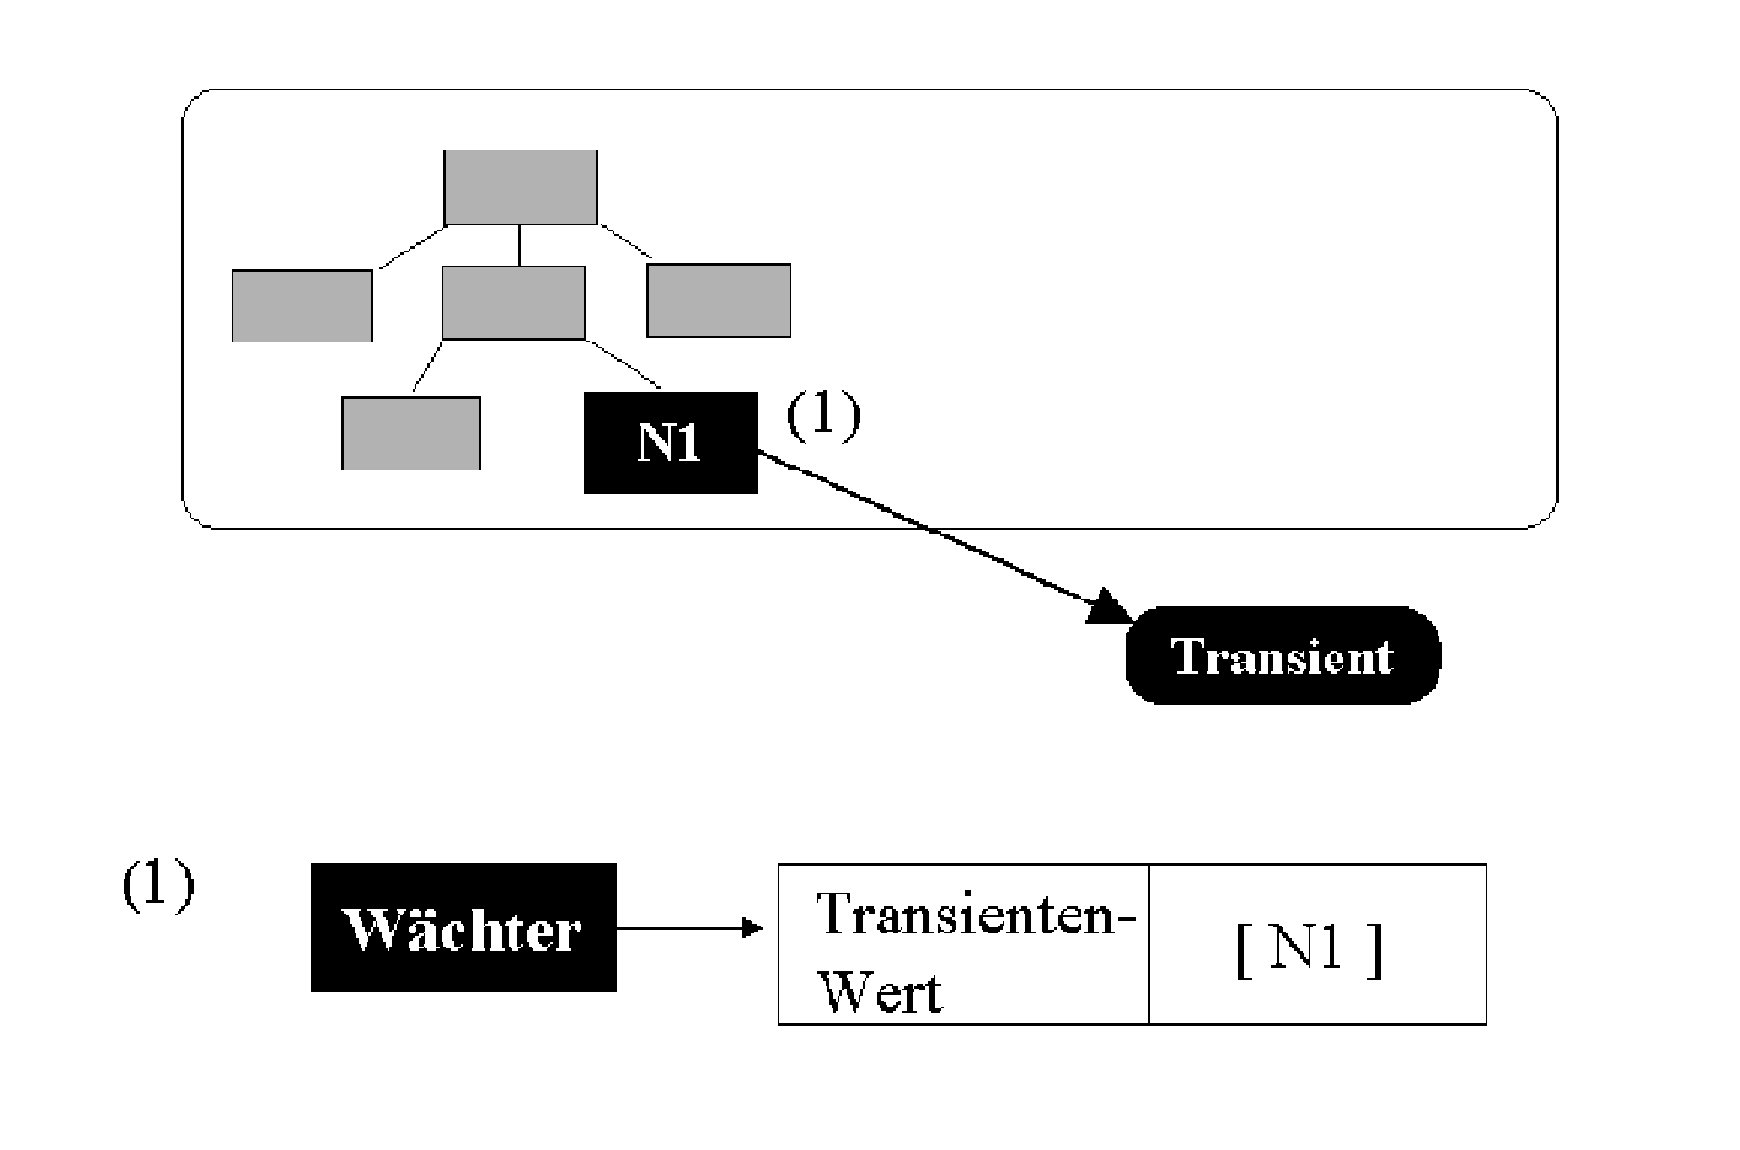
\epsfig{file = transient1_bw.ps, width = 12cm}
\linebreak 
Abbildung 3.6: Transient mit W\"{a}chter
\end{center}

\begin{center}
\epsfig{file = transient2_bw.ps, width = 12cm}
\linebreak 
Abbildung 3.7: Mehrfachauftreten des Transienten
\end{center}

\paragraph{}

Wurde der Transient, wie in Abbildung 3.8 dargestellt, schlie\ss lich
an einen Wert gebunden, hat der W\"achter nach der Ingangsetzung des
Aktualisierungsmechanismus' seine Funktion erf\"ullt und
wird beendet.

\begin{center}
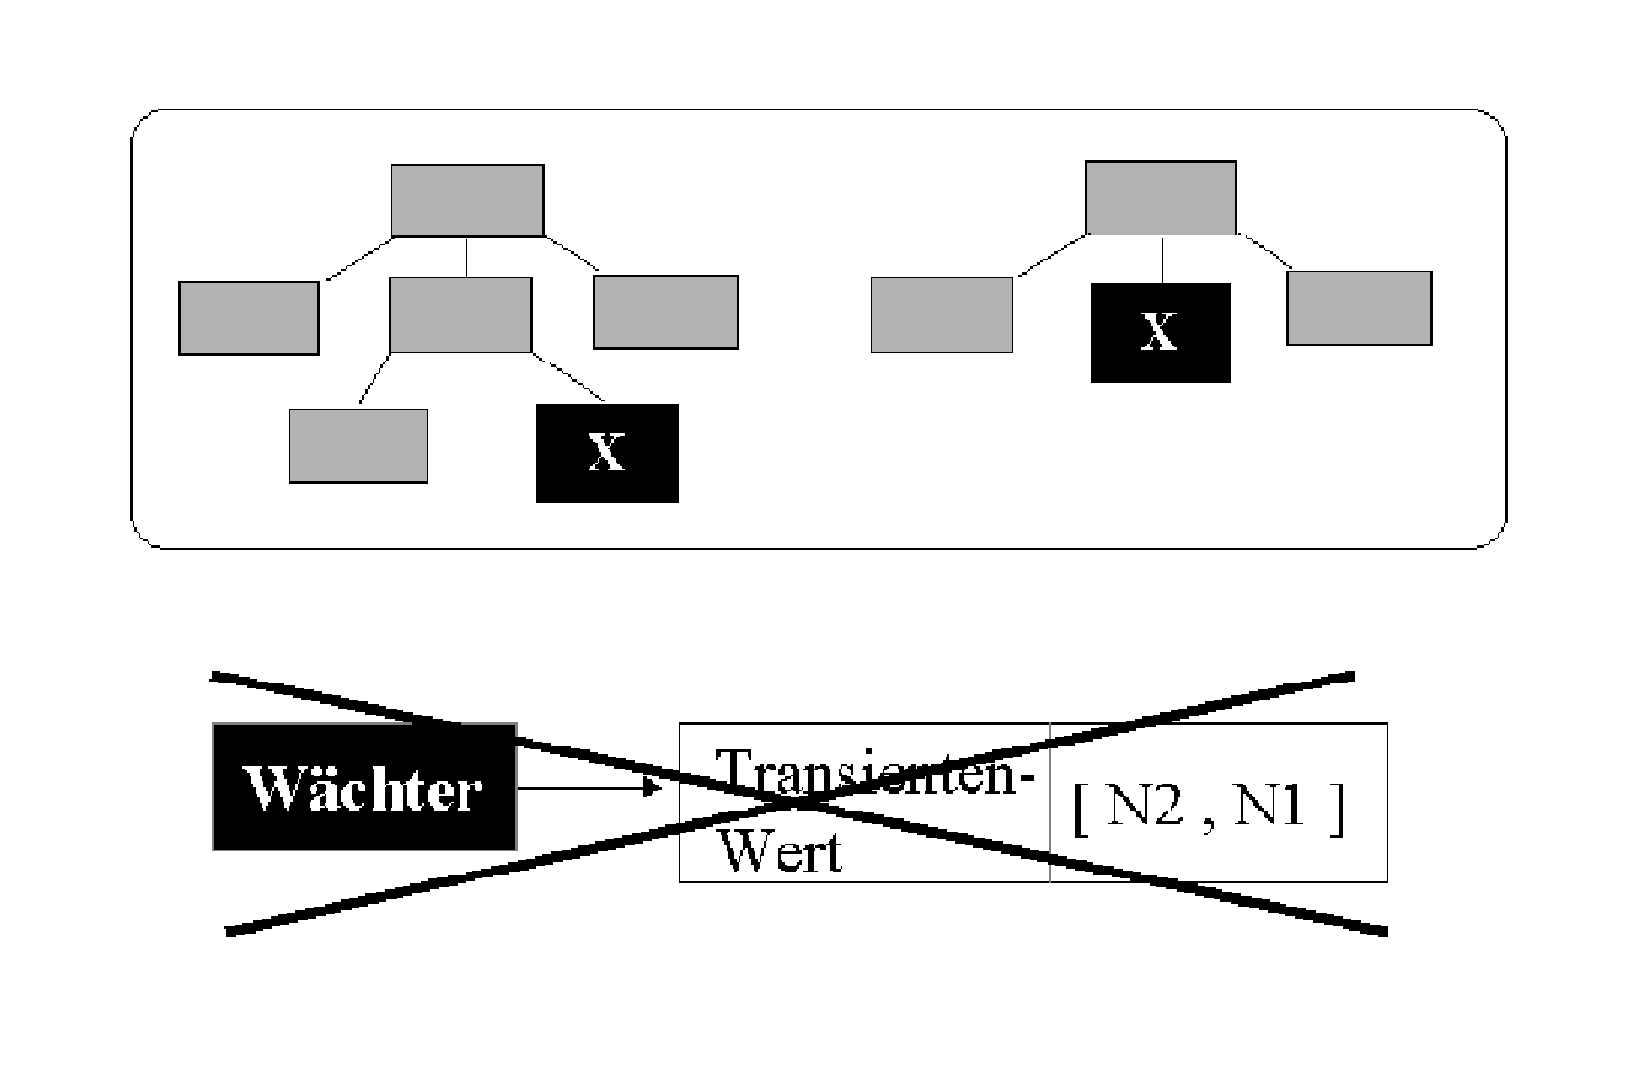
\epsfig{file = transient3_bw.ps, width = 12cm}
\linebreak 
Abbildung 3.8: Bindung des Transienten
\end{center}

\paragraph{}

Die oben beschriebene Aktualisierung der Darstellung erfolgt -
wie alle Darstellungsaktualisierungen - inkrementell. 
Dies bedeutet, dass - ausgehend  von der bestehenden Darstellung - 
nur m\"oglichst wenig Aufwand betrieben wird, um zu 
der neuen Darstellung zu gelangen. Nur diejenigen Teilb\"aume 
der internen Beschreibung werden neu konstruiert, gelayoutet und 
gezeichnet, f\"ur die dies unbedingt erforderlich ist. 


\subsection{Graphdarstellung}

\paragraph{}

Der Browser verf\"ugt \"uber den Graphmodus, in dem er token-Gleichheit -
physikalische Gleichheit von Objekten - innerhalb jeder dargestellten
Datenstruktur erkennt. Diesen Modus kann der Benutzer beliebig ein- und
ausschalten. Im Graphmodus ist die interne Darstellung von Werten 
nicht mehr baumartig [\ref{intern}], sondern graphartig aufgebaut.
Die Graphdarstellung eignet sich besonders zur Verbesserung der
\"Ubersichtlichkeit bei der Darstellung zyklischer Datenstrukturen. 

\paragraph{}

Betrachten wir den folgenden Datentypen: \newline
datatype tree = T of tree * tree. \newline
Die Deklaration \newline
 val rec t = T(t,t)  \newline
erzeugt einen unendlichen bin\"aren Baum. 
Die Baumdarstellung dieses Wertes 
enth\"alt f\"ur jeden Knoten  
eine eigene Repr\"asentation des jeweilgen Wertes, 
ohne die zyklische Struktur des Baumes zu beachten. 
Dagegen wird bei der Erzeugung der internen graphartigen
Darstellung der Zyklus erkannt, so dass ein endlicher zyklischer
Graph, wie in Abbildung 3.9 gezeigt, entsteht. 

\begin{center}
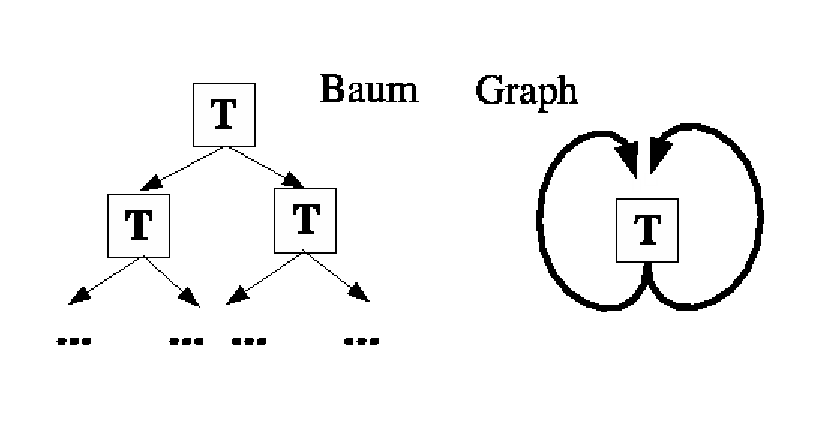
\epsfig{file = baum_graph.eps, width = 11cm}
\linebreak 
Abbildung 3.9: Baumdarstellung vs. Graphdarstellung
\end{center}


\subsection{Filter}

\paragraph{}

Der Browser muss in der Lage sein, den Umfang  der Darstellung zu begrenzen. 
Dies erlaubt dem Benutzer, die Darstellung auf das Wesentliche 
einzuschr\"anken. Weiterhin bietet ein Filter die M\"oglichkeit, 
die Darstellung zu gro\ss er oder zyklischer Datenstrukturen 
gem\"a\ss \, einer vom Benutzer gesetzten Grenze zu beschr\"anken. 
Die Definition von doc' (also auch von doc) wird dazu um die 
Variante ``limit'' erweitert.
erweitert (siehe Abbildung 3.10). \\[1mm]

\begin{minipage}{15cm}
\begin{math}
doc :=  simple \newline
\hspace*{8mm} | \quad  doc_{1} \quad \hat{} \quad ... \quad \hat{} 
                \quad  doc_{n} \newline   
\hspace*{8mm} | \quad  
\# \lbrack doc_{1}, ... , doc_{n}\rbrack \newline
\hspace*{8mm} | \quad limit 
\end{math} \newline
\end{minipage}
Abbildung 3.10: Erweiterung von doc' um ``limit''

\paragraph{}

Bei der internen Beschreibung, die der Browser f\"ur die 
Datenstrukturen erzeugt, kann die Tiefe der B\"aume beschr\"ankt werden 
(sogenanntes Tiefenlimit), sowie auch die jeweilige 
Anzahl konkatenierter oder akkumulierter Kinder, die ein Knoten haben 
darf (sogenanntes Breitenlimit). Wird bei der Erzeugung der internen 
Darstellung das Tiefen- oder Breitenlimit \"uberschritten, so wird an 
dieser Stelle die Konstruktion abgebrochen, und es wird ein ``limit'' 
angeh\"angt. Folglich handelt es sich bei ``limits'' in der Baumdarstellung 
stets um Bl\"atter. Den Abbruch des Aufbaus der internen Darstellung und 
das Setzen eines ``limits'' an die entsprechende Stelle bezeichnet man 
als Filtern. 

\paragraph{}

In der Browserdarstellung wird das \"Uberschreiten des
Tiefen- oder Breitenlimits an der entsprechenden Stelle durch einen Pfeil
gekennzeichnet. 


%%% IMPLEMENTIERUNG ====================================================

\section{Implementierung}

\subsection{Knotentypen}

\paragraph{}

F\"ur die Betrachtung des Designs gen\"ugt es, 
die aus den Werten erzeugte Beschreibung als doc darzustellen. 
In der Praxis m\"ochte man diese doc-Knoten aber um zus\"atzliche 
Attribute erweitern, wie beispielsweise die von der 
Anordnungsberechnung erzeugte Information und die Gtk-Gruppierung,
die vom Zeichenmechanismus ben\"otigt werden. 

\paragraph{}

Daher gibt es in der Implementierung zwei Datentypen, 
die die interne Beschreibung von Alice-Werten darstellen. 
Der erste - doc' - stellt die Benutzerschnittstelle f\"ur 
die Registrierung abstrakter Typen dar und ist daher auf das 
Wesentliche beschr\"ankt. Jedes Konstrukt diese Datentyps speichert 
im Wesentlichen nur den Wert, den es repr\"asentiert, und seinen
reflektierten Typen. 

\paragraph{}

Da alle Werte letztendlich in Konstukte des Datentyps doc transformiert
werden, besitzt doc in der Implementierung noch zus\"atzliche Felder, 
sogenannte ``Zust\"ande''.
Diese enthalten neben Anordnungsinformationen noch weitere Informationen,
die f\"ur ds Zeichnen der Werte auf die Benuteroberfl\"ache und f\"ur die
Aktualiesierung bereits dargestellter Werte von Nutzen sind.

\begin{center}
\begin{verbatim}
  datatype doc' = 
        
        SIMPLE of {desc : desc, 
                   rep : string, 
                   color : color_class }
        
      | CONCAT of {desc : desc, 
                   kids : doc vector }
        
      | CONTAINER of {desc : desc, 
                      kids : doc vector }
        
      | LIMIT of {desc : desc, 
                  sort : limit }
        
      | EMBEDDED of Reflect.value * Type.t  

\end{verbatim}  
Abbildung 4.1: Datentyp doc'
\end{center}

\paragraph{}

Abbildung 4.1 zeigt die Implementierung des Datentyps
doc'. Die ``SIMPLES'' stellen atomare Alice-Werte oder Trennzeichen dar. 
Diese k\"onnen durch einen String repr\"{a}sentiert werden. 
Au\ss erdem kann ihnen eine Farbe zugewiesen werden, in der sie 
auf die Benutzeroberfl\"ache gezeichnet werden. 
Der abstrakte Typ desc dient dazu, Wert und Typ einzukapseln - das
Speichern von Wert und Typ ist n\"otig, um bei der \"Anderung 
der Darstellung nochmal darauf zugreifen zu k\"onnen.
``CONCATS'' und ``CONTAINER'' stellen Konkatenation  
und Akkumulation von mehreren doc'-Knoten dar. 
``LIMITS'' markieren das \"Uberschreiten der 
vom Benutzer einstellbaren Begrenzungen. Das Feld 
``sort'' gibt dabei an, ob die maximal erlaubte Darstellungstiefe
oder -breite \"uberschritten wurde.

\paragraph{}

``EMBEDDEDS'' stellen Wert-Typ-Paare dar, die von einer Prozedur nicht
weiter bearbeitet werden konnten und deshalb in dieser Form an die
n\"achste, daf\"ur zust\"andige, Prozedur weitergereicht werden.
Dabei wird allen Alice-Werten durch Reflektion der Typ Reflect.value
gegeben. Das hat den Vorteil, dass der Datentyp doc' nicht polymorph
als 'a doc' deklariert werden muss.


\subsection{Typregistrierung und -zerlegung}

\paragraph{}

Abstrakte Typen enthalten zwar keine strukturelle Information \"uber 
Werte dieses Typs, jedoch existiert zu jedem abstrakten Typen ein sogenannter 
Pfad, der Informationen \"uber de Struktur von Werten dieses Typs enth\"alt.
Beim Registrieren eines abstrakten Typs beim Browser wird der Pfad des Typs 
zusammen mit der entsprechenden create-Prozedur, die Werte dieses Typs auf 
genau einer Ebene zerlegen kann und somit ein doc'-Konstrukt erzeugt, in einer 
Map gespeichert. Dabei wird jeweils der Pfad als Schl\"ussel benutzt.

\paragraph{} 

Der Browser enth\"alt bereits die n\"otigen Mechanismen, 
um Werte struktureller 
Typen in entsprechende Beschreibungen zu transformieren. 
Diese Mechanismen arbeiten die zu inspizierenden Werte 
struktureller Typen solange ab, bis sie auf einen Teilwert sto\ss en, der
einen abstrakten Typ hat. Zur weiteren Zerlegung extrahiert man nun den Pfad
des abstrakten Typs und sucht in der oben beschriebenen Map nach der passenden
create-Prozedur f\"ur Werte dieses Typs.  
Dieser wird dann der Wert zusammen mit seinem Typ zur weiteren Bearbeitung 
\"ubergeben.  Wird in der Map keine passende Prozedur gefunden, 
so wird ein Standardknoten erzeugt, der das Symbol \_ als 
Stringrepr\"asentation enth\"alt.

\paragraph{} 

Die Implementierung des Browsers beinhaltet desweiteren schon create- \newline
Prozeduren f\"ur gebr\"auchliche abstrakte Typen wie beispielsweise 
Array, Vektor, Referenz, Int, String, Real, etc.
Au\ss erdem stehen dem create-Mechanismus die notwendigen Hilfsprozeduren
zur Zerlegung struktureller Typen zur Verf\"ugung. Der create-Mechanismus 
f\"uhrt die Typzerlegung jeweils solange selbst\"andig durch, bis er auf einen 
abstrakten Typen st\"o\ss t. F\"ur diesen muss dann in der Map nach der
 passenden create-Prozedur gesucht werden. 
Insgesamt wird ein Wert also solange in Teilwerte zerlegt und gegebenfalls
zwischen verschiedenen Prozeduren hin- und hergereicht, bis er vollst\"andig
in die interne Beschreibung transformiert worden ist, d.h. bis aus dem
Wert ein doc-Konstrukt entstanden ist, dass keine unbearbeiteten 
Wert-Typ-Paare mehr enth\"alt.

\subsection{Layout}

\begin{center}
\begin{picture}(300,250)

\put(100,80){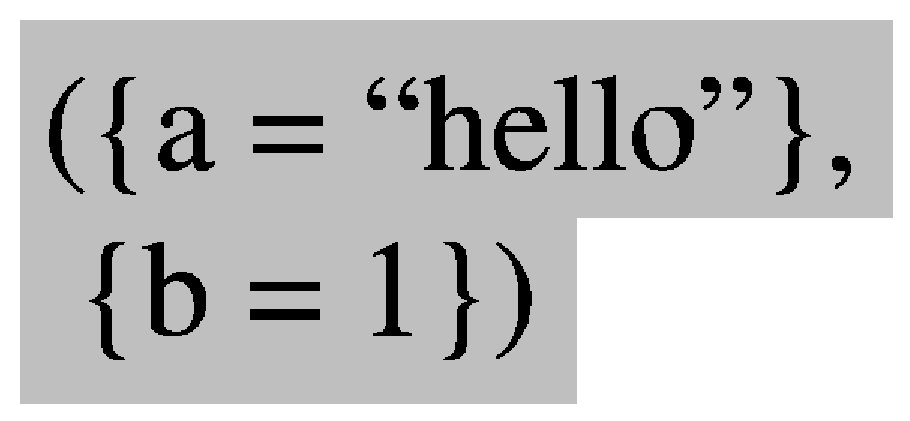
\epsfig{file = lay.eps, width = 200pt, height = 100pt}{}}

\put(100,50){\vector(4,0){130}}
\put(70,80){\vector(0,4){100}}
\put(100,210){\vector(4,0){200}}

\put(230,50){\vector(-4,0){130}}
\put(70,180){\vector(0,-4){100}}
\put(300,210){\vector(-4,0){200}}

\put(150,20){lxdim}
\put(0,130){ydim}
\put(150,250){xdim}

\end{picture} \newline
Abbildung 4.2: Bounding-Box einer Wertdarstellung
\end{center}

\paragraph{}

Die Anordnungsberechnung orientiert sich an den 
Varianten der Wertbeschreibung der darzustellenden 
Werte. Hierbei wird zwischen den Verkn\"upfungen 
Akkumulation und Konkatenation und atomaren 
Wertbeschreibungen unterschieden.

\paragraph{}

Die graphischen Repr\"{a}sentationen von 
Wertbeschreibungen, die \"{u}ber 
Akkumulation miteinander verkn\"{u}pft sind, 
werden abh\"{a}ngig davon, ob diese 
wiederum Verkn\"{u}pfungen enthalten, vertikal 
oder horizontal nebeneinander auf der Zeichenfl\"{a}che 
angeordnet. Nur in dem Fall, dass die 
Verkn\"{u}pfung keine weiteren Verkn\"{u}pfungen 
enth\"{a}lt, wird die horizontale Anordnung gew\"{a}hlt.

\paragraph{}

Die graphischen Repr\"{a}sentationen von Wertbeschreibungen, 
die mit Konkatenation verkn\"{u}pft sind, werden 
immer horizontal nebeneinander angeordnet. 

\paragraph{}

Die Anordnungsberechnung dient insbesondere 
dazu, die H\"{o}he und die Breite 
der Textdarstellung der darzustellenden Werte 
zu ermitteln sowie die Breite der jeweils 
letzten Zeile dieser Darstellung, wie in 
Abbildung 4.2 gezeigt. Dies 
entspricht der Berechnung der ``bounding box'' \cite{br:oz} 
einer Wertrepr\"{a}sentation. Die 
Berechnung erfolgt bottom-up unter Ber\"{u}cksichtigung 
der Anordnungsvorschriften.  

\subsection{Zeichnen}

\paragraph{}

Jedem Knoten der internen Beschreibung wird bereits bei seiner  
Erzeugung eine Gtk-Gruppe zugewiesen, 
die alle Unterb\"aume dieses Knotens beinhaltet. Die Gtk-Gruppen sind 
folglich  analog zu der Baumstruktur der internen Beschreibung hierarchisch 
geordnet. 
Nach der Erzeugung der internen Beschreibung und der Layout-Berechnung 
wird die Repr\"asentation der Datenstrukturen mittels top-down 
left-to-right-Traverierung auf die Zeichenfl\"ache der 
Benutzerschnittstelle gezeichnet. Die Textrepr\"asentationen eines 
Knotens werden dabei in die dazugeh\"orige Gruppe gesetzt. 


\subsection{Transientenverwaltung}

\paragraph{}

Der Browser erzeugt f\"ur jeden Transienten einen W\"achter-Thread, 
der darauf wartet, dass dieser an einen Wert gebunden
wird. Da der Browser mehrere Repr\"asentationen desselben 
Transienten erzeugen kann - z.B. durch wiederholtes Inspizieren - 
ist es sinnvoll, nur jeweils einen W\"achter pro Transient daf\"ur 
einzusetzen, der aber alle diesen Transienten darstellenden Knoten der 
internen Beschreibung kennen muss.
Dazu gibt es ein sogenanntes Transienten-Dictionary, in dem 
jeweils Tripel, bestehend aus dem inspizierten Transienten-Wert, 
einem dazugeh\"origen W\"achter-Thread, und einer 
Liste aller Knoten, die auf diesen Transienten verweisen, 
gespeichert sind. Abbildung 4.3 zeigt die Form eines 
Dictionary-Eintrages.
\begin{center}
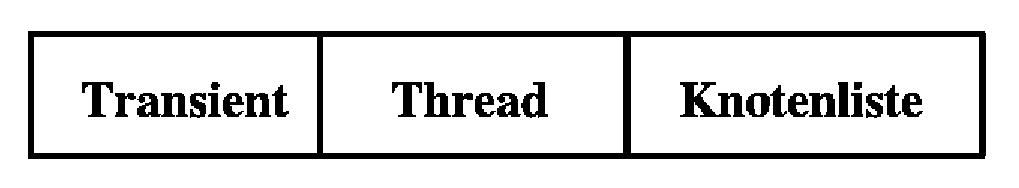
\epsfig{file = transdict.eps, width = 6cm}
\newline Abbildung 4.3: Eintrag im Transienten-Dictionary
\end{center}

Der W\"achter-Thread reagiert auf die Wertzuweisung 
an den von ihm \"uberwachten Transienten und aktualisiert 
die Darstellung. Dabei m\"ussen die Tranisenten-Knoten 
der Beschreibung durch die Repr\"asentationen der neuen 
Werte ersetzt werden. Dies geschieht inkrementell [\ref{inkr}].


\subsection{Inkrementalit\"at}

\label{inkr} 

\paragraph{}

Die Darstellung der inspizierten Alice-Werte auf 
der graphischen Benutzeroberfl\"ache muss 
schnell an Ver\"anderungen der inspizierten 
Werte angepasst werden k\"onnen. Dies 
wird unter anderem dann erforderlich, wenn 
eine Wertzuweisung an einen Transienten 
erfolgt, so dass die Darstellung des 
neuen Wertes die Darstellung des Transienten 
auf der Benutzeroberfl\"ache ersetzen soll. 
Diese Ver\"anderungen erfolgen inkrementell, 
d.h. ausgehend von der bereits bestehenden 
Darstellung wird m\"oglichst wenig Berechnungsaufwand 
betrieben, um zur neuen Darstellung zu gelangen.

\begin{center}
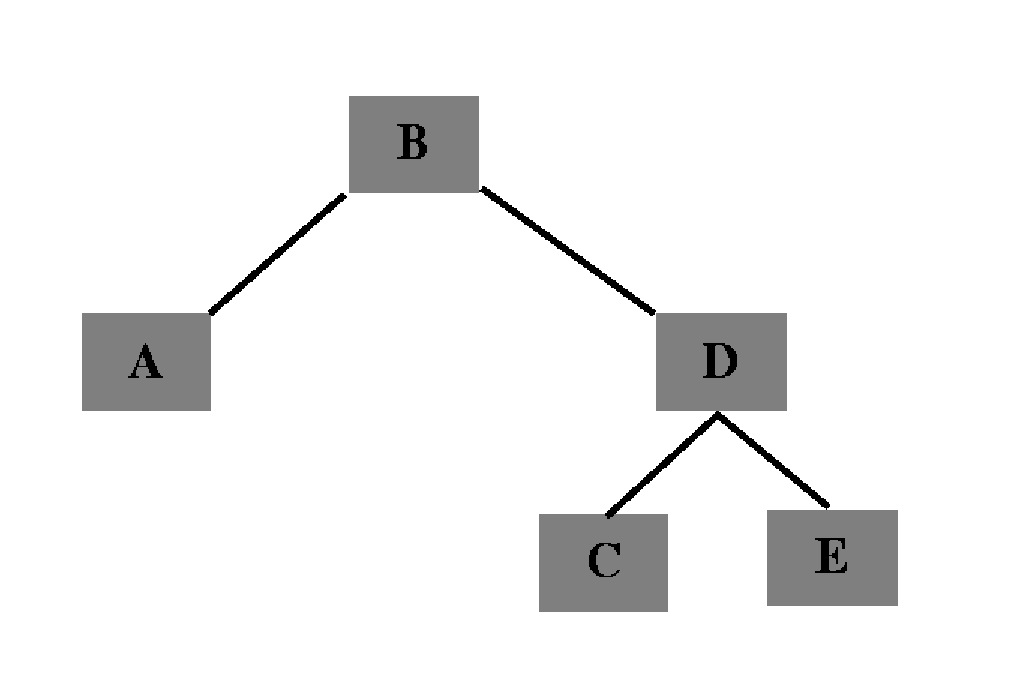
\epsfig{file = inkrem1.eps, width = 10cm}
\newline Abbildung 4.4: interne Beschreibung (stark vereinfacht)
\end{center} 

Abbildung 4.4 stellt die interne (baumartige) Beschreibung einer 
Datenstruktur dar. Es wird angenommen, dass die Darstellung 
des durch Knoten A repr\"{a}sentierten 
Wertes ersetzt werden muss.

\begin{center}
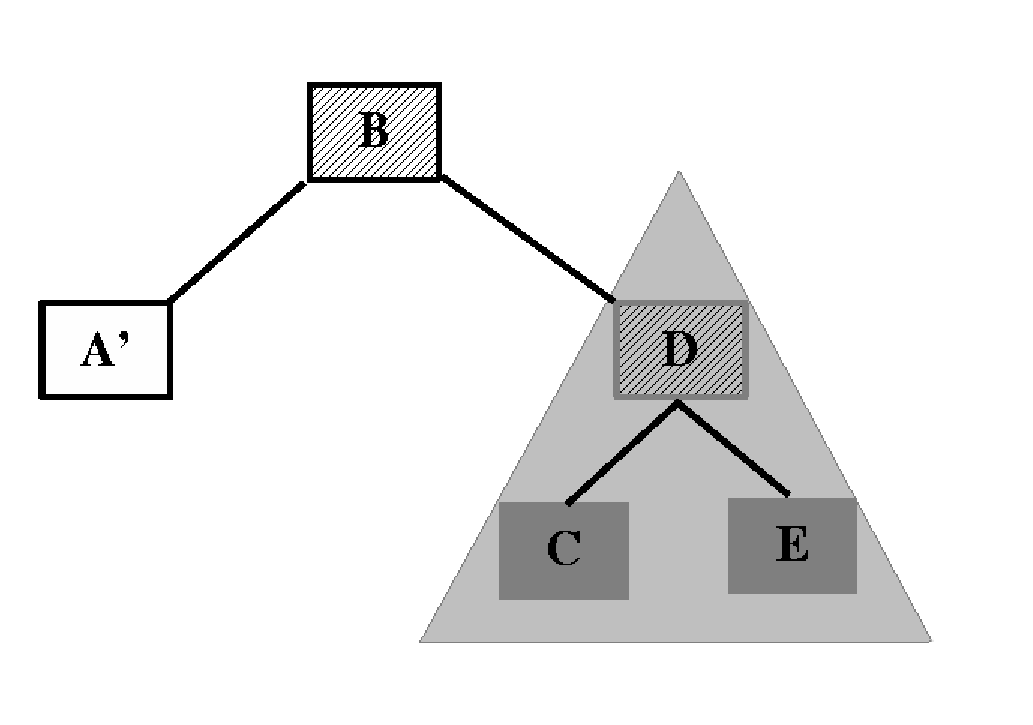
\epsfig{file = inkrem2.eps, width = 10cm}
\newline Abbildung 4.5: inkrementelle Ver\"anderung 
\end{center}


Abbildung 4.5 zeigt die n\"otigen Schritte, um 
zu einer 
neuen Beschreibung und zu einer neuen Darstellung 
auf der Benutzeroberfl\"ache zu gelangen. 
Der betroffene Teilbaum selbst, hier der Knoten A', 
 muss vollkommen neu konstruiert 
und angeordnet werden, und dessen graphische Repr\"asentation 
muss neu gezeichnet werden. Da dies die Anordnung der 
graohischen Repr\"asentationen der gesamten 
baumartigen Beschreibung st\"oren kann, muss auf dem Pfad von 
diesem Teilbaum zum Wurzelknoten die Anordnung neu berechnet werden. 
In diesem Beispiel betrifft das den Knoten B.
Dies kann zur Folge haben, dass die Textdarstellungen 
der von der \"Anderung nicht direkt 
betroffene Teilb\"aume an neue Positionen verschoben 
werden m\"ussen. Von diesen Positions\"{a}nderungen 
abgesehen k\"onnen diese Teilb\"aume unver\"andert 
beibehalten werden.
In dem Beispiel m\"ussen die textuellen Repr\"asentationen
des Teilbaums {C,D,E} auf der graphischen Benutzeroberfl\"ache 
verschoben werden.
Das ist g\"unstiger, als den gesamten 
Baum neu zu konstruieren, anzuordnen und zu zeichnen.   
 

\subsection{Module}

\begin{center}
\epsfig{file = module_bw.ps, width = 13cm}
\linebreak Abbildung 4.6: Module des Browsers
\end{center}

Abbildung 4.6 zeigt die Module des Browsers.
Dieser verf\"{u}gt \"{u}ber zwei Module, die 
die Datentypen der internen Beschreibung  - doc' und doc - enthalten.
Das Modul Doc enth\"alt doc', und Node ent\"alt doc.
Neben den Datentypen beinhalten die Module \"{u}ber 
entsprechende Accessoren.
Da diese w\"{a}hrend der 
Erzeugnung, der Anordnungsberechnung, dem Zeichnen 
und der Darstellungsab\"{a}nderung verwendet werden, 
werden diese Module in vielen anderen Modulen benutzt.\\
Das Modul GtkSupport kapselt die Gtk-Funktionalit\"{a}t 
gegen\"{u}ber allen anderen Modulen des Browsers ab. 
Als einziges Modul hat es direkten Zugriff auf die 
Gtk-Prozeduren. Die anderen Module des Browsers 
greifen dabei auf GtkSupport zur\"{u}ck.
Die Module CreateTree, Layout, und Draw repr\"{a}sentieren 
die drei Phasen des Inspektionsvorgangs, w\"ahrend das Modul 
Update die notwendigen Mechanismen repr\"asentiert, 
um die Darstellung an Ver\"{a}nderungen anzupassen. 
Das Modul Widget verf\"{u}gt \"{u}ber die 
graphische Benutzeroberfl\"{a}che und steuert 
die Darstellungserzeugung bzw. Ver\"{a}nderung. 
Letztendlich macht das Modul UnsafeInspector die f\"{u}r den 
Benutzer relevanten Prozeduren und Datentypen nach au\ss en sichtbar.


%%% AUSBLICK ===========================================================

\section{Ausblick}

\paragraph{}

Zur Zeit verwenden wir ein Gtk-Binding f\"ur Mozart \cite{mo:mo}
zur Erzeugung der graphischen Benutzeroberfl\"ache. Allerdings ist 
es auch m\"oglich, den Browser an eine von Robert Grabowski im Rahmen 
seines Fortgeschrittenenpraktikums neu implementierte Gtk-Schnittstelle
f\"ur Alice \cite{gr:gt} anzuschlie\ss en.

\paragraph{}

Desweiteren ist der Alice-Browser nicht typsicher, 
da der Benutzer zur Zeit ein Tupel aus 
Wert und mithilfe des Typreflektors reflektierten Typs 
an die inspect-Funktion \"ubergibt.  
Eine automatische Typreflektion w\"urde die Benutzung des Tools 
erleichtern und eine Fehlbenutzung ausschlie\ss en. 
In diesem Fall m\"usste der Benutzer nur noch den zu 
inspizierenden Wert \"ubergeben. 

\paragraph{}

Mithilfe eines \"ubergeordneten Funktors lie\ss e 
sich der Browser einkapseln.


%%% BIBLIOGRAPHIE =======================================================

\begin{thebibliography}{99}

\bibitem{br:oz} Thorsten Brunklaus 2000. {\em Der Oz Inspector - Browsen: 
    Interaktiver, einfacher, effizienter}. Diplomarbeit, Universit\"at 
    des Saarlandes, Fachbereich Informatik.
\bibitem{op:pr} Derek Oppen 1980. {\em Prettyprinting}. ACM Transactions 
  on Programming Languages and Systems, Bd. 2, Nr. 4, 1980, pp 465-483.
\bibitem{ke:dr} Andrew Kennedy 1996. {\em Drawing Trees}. 
                Journal of Functional Programming, Bd. 6(3), pp. 527-534.
\bibitem{al:al} Alice-Homepage. {\em www.ps.uni-sb.de/alice/}
\bibitem{gt:gt} GTK+: The Gimp Toolkit.{\em www.gtk.org}. 
\bibitem{mo:mo} The Mozart Programming System. {\em www.mozart-oz.org/}.
\bibitem{gr:gt} Robert Grabowski 2003. {\em Eine Gtk-Schnittstelle f\"ur 
                Alice}. 
                FoPra-Ausarbeitung, Lehrstuhl Prof. G. Smolka, 
                Universtit\"at des Saarlandes.

\end{thebibliography}

\end{document}

















